\documentclass[12pt,a4paper]{article}

% --- KHAI BÁO PACKAGES (Từ Bản 2) ---
% --- NHÓM CẤU HÌNH CƠ BẢN ---
\usepackage[utf8]{inputenc}
\usepackage[T1]{fontenc}
\usepackage[a4paper,margin=1in]{geometry}
\usepackage{graphicx}
\usepackage{titlesec}
\usepackage{hyperref}
\usepackage{enumitem}
\usepackage{float}
\usepackage{caption}
\usepackage{booktabs}
\usepackage{setspace}
\usepackage{pifont}
\usepackage{amsmath} % Hỗ trợ công thức toán học
\usepackage{subcaption}
\usepackage{multirow}
\usepackage{pdfpages} % Thêm dòng này ở phần Preamble
\usepackage{tikz}
\usetikzlibrary{shapes.geometric, arrows, positioning}
\usepackage{hyperref}

% Định nghĩa các style cho khối sơ đồ
\tikzstyle{startstop} = [rectangle, rounded corners, minimum width=3cm, minimum height=1cm,text centered, draw=black, fill=red!30]
\tikzstyle{process} = [rectangle, minimum width=3cm, minimum height=1cm, text centered, draw=black, fill=orange!30]
\tikzstyle{decision} = [diamond, minimum width=3cm, minimum height=1cm, text centered, draw=black, fill=green!30]
\tikzstyle{arrow} = [thick,->,>=stealth]

% --- NHÓM ĐỊNH DẠNG CODE & KHUNG (Đã gộp & xóa trùng) ---
\usepackage{listings}
\usepackage{xcolor}
\usepackage{mdframed} 

% --- CẤU HÌNH MÀU SẮC & LISTINGS ---
\definecolor{codegreen}{rgb}{0,0.6,0}
\definecolor{codepurple}{rgb}{0.58,0,0.82}
\definecolor{backcolour}{rgb}{0.96,0.96,0.96}
\definecolor{codeblue}{rgb}{0.1,0.1,0.9}

\lstset{
    backgroundcolor=\color{backcolour},   
    commentstyle=\color{codegreen},
    keywordstyle=\color{codeblue}\bfseries,
    numberstyle=\tiny\color{gray},
    stringstyle=\color{codepurple},
    basicstyle=\ttfamily\small, 
    breakatwhitespace=false,         
    breaklines=true,                 
    captionpos=t,                    
    keepspaces=true,                 
    numbers=left,                    
    numbersep=8pt,                  
    showspaces=false,                
    showstringspaces=false,
    showtabs=false,                  
    tabsize=2,
    frame=tlbr, 
    framesep=5pt,
    framerule=0pt,
}

% Cấu hình bo góc cho khung code
\surroundwithmdframed[
    linecolor=lightgray,
    innerleftmargin=5pt,
    innerrightmargin=5pt,
    innertopmargin=0pt,
    innerbottommargin=0pt,
    roundcorner=5pt, 
    backgroundcolor=backcolour
]{lstlisting}

% --- CẤU HÌNH TRÌNH BÀY ---
\setlength{\parskip}{0.5em}
\setlength{\parindent}{0pt}
\setstretch{1.15}

\hypersetup{
    colorlinks=true,
    linkcolor=blue,
    urlcolor=cyan
}

\titleformat{\section}{\bfseries\large}{\thesection.}{1em}{}
\titleformat{\subsection}{\bfseries}{\thesubsection}{1em}{}


\begin{document}

% Chèn file PDF khác vào đầu
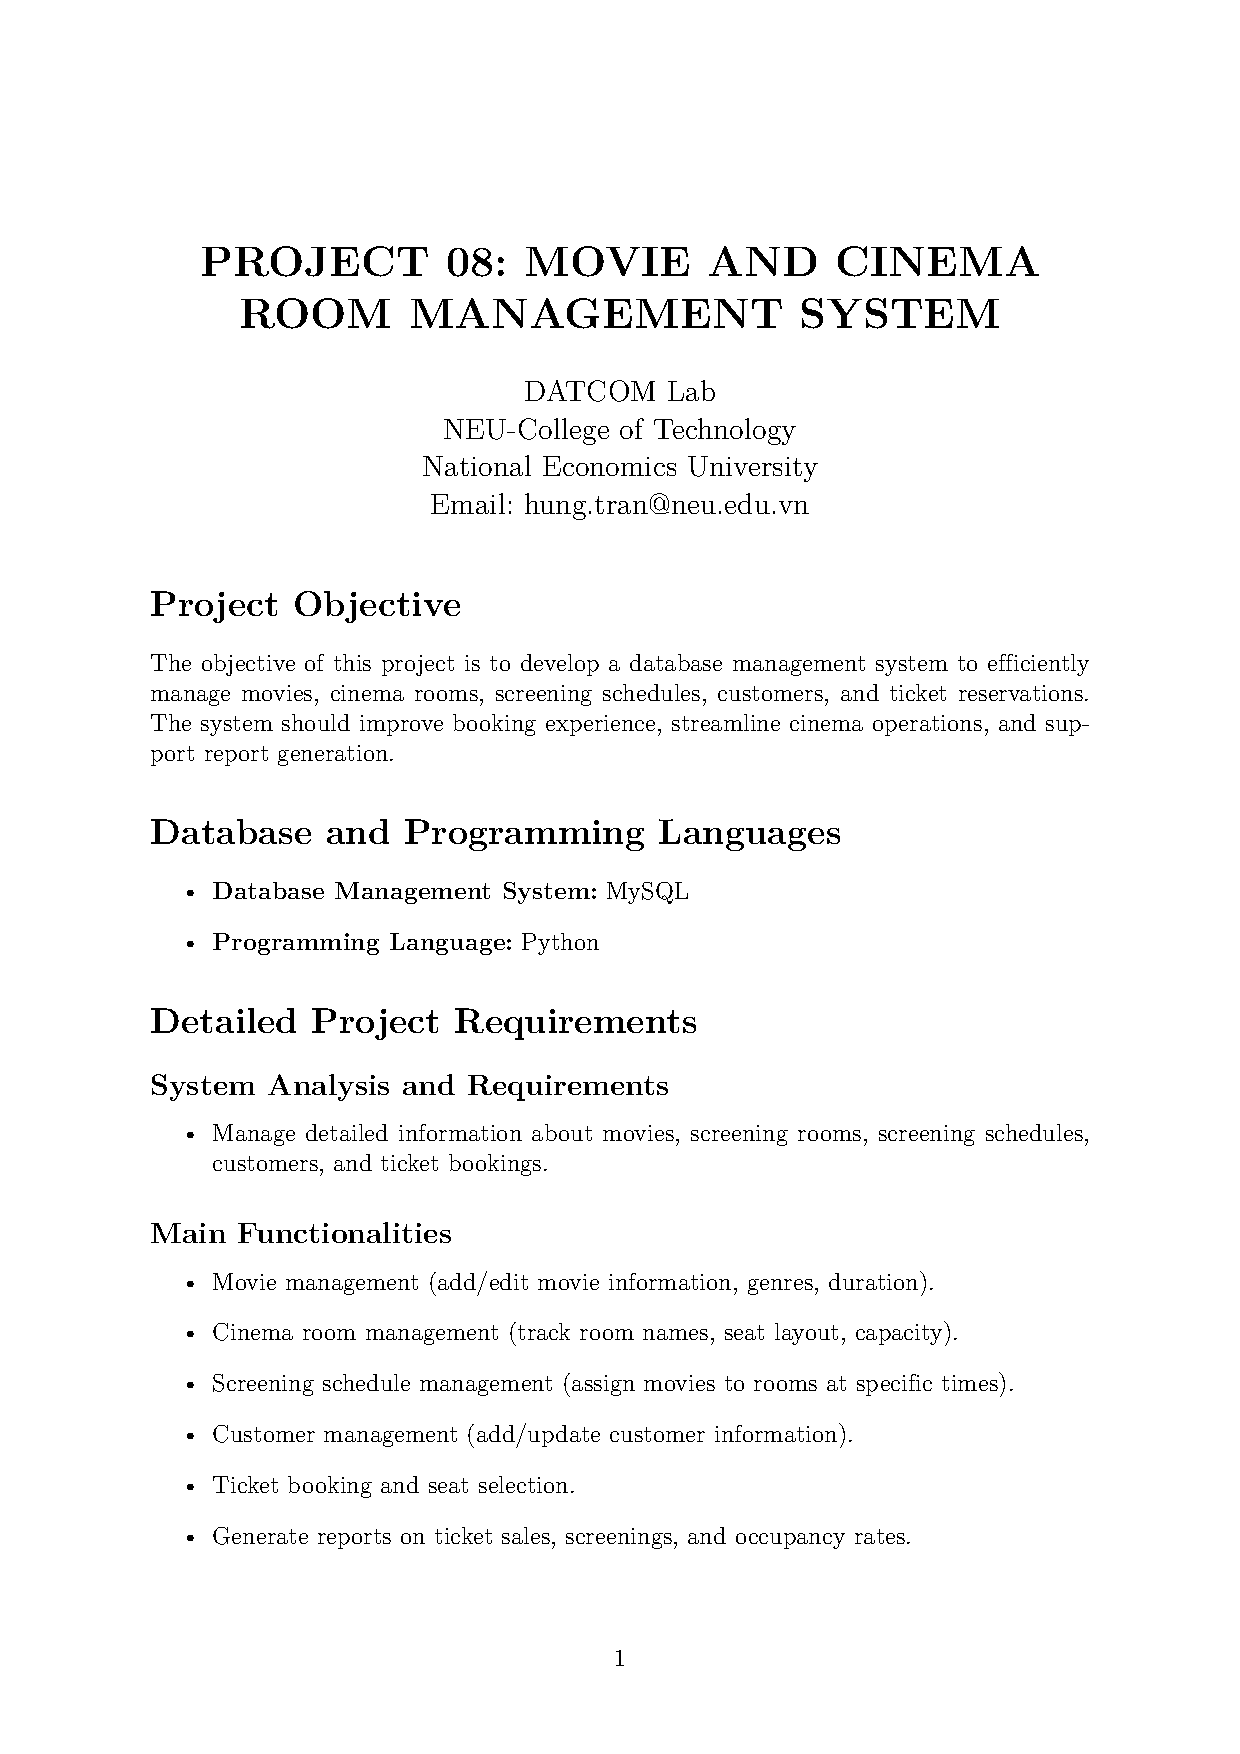
\includepdf[pages=-]{8.pdf}
% =====================================================
% TRANG BÌA (Design theo Bản 1)
% =====================================================
\begin{titlepage}
\begin{center}
    {\large \textbf{NATIONAL ECONOMICS UNIVERSITY, HANOI}} \\
    {\large \textbf{COLLEGE OF TECHNOLOGY}} \\
    {\small \textbf{FACULTY OF DATA SCIENCE AND ARTIFICIAL INTELLIGENCE}} \\
    
    \vspace{1.5cm}
    
    % Chú ý đường dẫn ảnh Images/
    
\includegraphics[width=4cm]{Images/NEU logo.png} 
    
    \vspace{1.5cm}
    
    \begin{center}
        \setstretch{1.5} % Giãn dòng một chút cho thoáng
        \begin{tabular}{p{0.9\linewidth}} % Định dạng cột rộng 90% chiều ngang trang giấy
            \hline
            \\[-0.2cm]
            \centering \textbf{\Large INTRODUCTION TO DATABASES} \\[0.3cm]
            \centering \textbf{\Large REPORT} \\[0.5cm]
            
            % Phần Topic dùng minipage để tự động xuống dòng và căn giữa
            \centering \begin{minipage}{0.85\linewidth}
                \centering \textbf{\Large Topic: MOVIE AND CINEMA ROOM MANAGEMENT SYSTEM}
            \end{minipage} \\[0.8cm]
            

        \end{tabular}
    \end{center}

    \vspace{2cm}

            % Thông tin sinh viên - Căn chỉnh lại để không lỗi font
    \begin{table}[h]
        \centering
        \begin{tabular}{ll}
            \textbf{Student:} & Nguyen Thi Hai Yen \\
            \textbf{Student ID:} & 11247252 \\
            \textbf{Major:} & Data Science \\
            \textbf{Supervisor:} & Tran Hung \\
        \end{tabular}
    \end{table}

    \vspace{2cm}
            
            % Ngày tháng
    {\small Hanoi, \today}
            
\end{center}
\end{titlepage}

% =====================================================
% MỤC LỤC
% =====================================================
\pagenumbering{roman}
\tableofcontents
\newpage
\listoffigures % Đưa lên đây để dùng số trang La Mã
\newpage

\listoftables % Đưa lên đây luôn cho đồng bộ
\newpage

\pagenumbering{arabic}
\setcounter{page}{1} % Đảm bảo nội dung chính bắt đầu đúng từ trang 1

% =====================================================
% NỘI DUNG (Cấu trúc của Bản 2)
% =====================================================

\section{Introduction}
\input{2-Intro.text} 

\section{Methodology}
\input{3-Method.text}

\section{Conclusion}
\input{4-Conclusion.text}

\section{Discussion}
\input{5-Discuss.text}

\end{document}